\documentclass[12pt, twoside]{article}
%\documentclass[12pt, twoside]{article}
\usepackage[letterpaper, margin=1in, headsep=0.2in]{geometry}
\setlength{\headheight}{0.6in}
%\usepackage[english]{babel}
\usepackage[utf8]{inputenc}
\usepackage{microtype}
\usepackage{amsmath}
\usepackage{amssymb}
%\usepackage{amsfonts}
\usepackage[nomessages]{fp} %\FPeval{\var-name}{2*sin(pi/6)}
\usepackage{siunitx} %units in math. eg 20\milli\meter
\usepackage{yhmath} % for arcs, overparenth command
\usepackage{tikz} %graphics
\usetikzlibrary{quotes, angles, arrows, arrows.meta}
\usepackage{pgfplots}
\usepgfplotslibrary{fillbetween}
\pgfplotsset{compat=1.16}
\usepackage{graphicx} %consider setting \graphicspath{{images/}}
\usepackage{parskip} %no paragraph indent
\usepackage{enumitem}
\usepackage{multicol}
\usepackage{venndiagram}

\usepackage{fancyhdr}
\pagestyle{fancy}
\fancyhf{}
\renewcommand{\headrulewidth}{0pt} % disable the underline of the header
\raggedbottom
\hfuzz=2mm %suppresses overfull box warnings

\usepackage{hyperref}

% Number line from -5 to 5 for students to draw on, or with a drawn set.
\newcommand{\numline}[1]{%
\begin{tikzpicture}[scale=0.68, baseline=-3pt]
  \draw[thick, <->] (-5.6,0) -- (5.6,0) node[right] {$x$};
  \foreach \x in {-5,...,5} {\draw (\x,0.12) -- (\x,-0.12) node[below] {\footnotesize $\x$};}
  #1
\end{tikzpicture}}
\newcommand{\closeddot}[1]{\fill (#1,0) circle (0.13);}
\newcommand{\opendot}[1]{\filldraw[fill=white, thick] (#1,0) circle (0.13);}

\fancyhead[LO]{La Scuola d'Italia / Dr.\ Huson / IB Math 11 \\* 11 November 2026}
\fancyhead[RO]{\fbox{\begin{minipage}{6cm}\footnotesize Nickname:\\[0.5cm]\end{minipage}}}
\fancyfoot[C]{\thepage}

\begin{document}
\subsubsection*{3.1 Classwork: Sets and Venn Diagrams Review (no calculator)}

\begin{center}
\small
\renewcommand{\arraystretch}{1.2}
\begin{tabular}{|c|l||c|l|}
\hline
$x \in A$ & $x$ is an element of $A$ & $A \cap B$ & intersection: in $A$ \emph{and} in $B$ \\
$x \notin A$ & $x$ is not an element of $A$ & $A \cup B$ & union: in $A$ \emph{or} $B$ (or both) \\
$n(A)$ & the number of elements in $A$ & $A'$ & complement: not in $A$ \\
$A \subseteq B$ & $A$ is a subset of $B$ & $U$ & the universal set \\
$\varnothing$ & the empty set, $\{\ \}$ & $\{x \mid \ldots\}$ & the set of all $x$ such that \ldots \\
\hline
\end{tabular}
\end{center}

\begin{enumerate}[itemsep=0.15cm]

%--- Problem 1: Primes as a set: list primes < 30, n(P); true/false with element and subset notation; factors of 30 intersect primes; finite or infinite [13 marks] ---
%--- Source: Original (Haese Core Topics SL 2A-2B; prior learning); prime-number reminder at Chris's request ---
\item[1.]
A \emph{prime number} is a positive integer with exactly two positive factors:
$1$ and itself. So $1$ is \emph{not} prime.

Let $P = \{\text{prime numbers less than } 30\}$.

\begin{enumerate}[itemsep=0.15cm]
  \item List the elements of $P$, and write down $n(P)$. \vfill
  \item Write down the only even prime number. Explain why every other
  even number is not prime. \vfill
  \item State whether each statement is true or false.

  \begin{tabular}{@{}p{0.13\textwidth}p{0.13\textwidth}p{0.13\textwidth}p{0.2\textwidth}p{0.15\textwidth}}
  (i) $9 \in P$ & (ii) $2 \in P$ & (iii) $1 \in P$ &
  (iv) $\{3, 5\} \subseteq P$ & (v) $27 \notin P$
  \end{tabular}
  \vfill
  \item Let $F = \{\text{positive factors of } 30\}$. List the elements of
  $F$, and find $F \cap P$. Describe $F \cap P$ in words. \vfill
  \item Is the set of \emph{all} prime numbers finite or infinite? \vfill
\end{enumerate}

\newpage

%--- Problem 2: Special number sets N, Z, Z+, Q, R: true/false; place eight numbers in a nested Venn diagram [12 marks] ---
%--- Source: Original (Haese Core Topics SL 2D, Exercise 2D Q2-3, 2F Q6) ---
\item[2.]
$\mathbb{N} = \{0, 1, 2, 3, \ldots\}$, \quad
$\mathbb{Z} = \{0, \pm 1, \pm 2, \ldots\}$, \quad
$\mathbb{Z}^{+} = \{1, 2, 3, \ldots\}$, \quad
$\mathbb{Q}$ = rational numbers $\dfrac{p}{q}$ ($p, q \in \mathbb{Z}$,
$q \neq 0$), \quad $\mathbb{R}$ = real numbers.

\begin{enumerate}[itemsep=0.15cm]
  \item State whether each statement is true or false.

  \begin{tabular}{@{}p{0.2\textwidth}p{0.2\textwidth}p{0.2\textwidth}p{0.2\textwidth}}
  (i) $-3 \in \mathbb{N}$ & (ii) $0 \in \mathbb{N}$ & (iii) $0 \in \mathbb{Z}^{+}$ &
  (iv) $\sqrt{2} \in \mathbb{Q}$ \\[0.3cm]
  (v) $0.25 \in \mathbb{Q}$ & (vi) $0.\overline{3} \in \mathbb{Q}$ &
  (vii) $\mathbb{Z} \subseteq \mathbb{Q}$ & (viii) $\mathbb{Q} \subseteq \mathbb{Z}$
  \end{tabular}
  \vfill
  \item Write each number in the correct region of the Venn diagram.
  \[
  7, \quad -2, \quad 0, \quad \frac{1}{3}, \quad -0.6, \quad \sqrt{16}, \quad
  \sqrt{5}, \quad \pi
  \]
  \begin{center}
  \begin{tikzpicture}
    \draw[thick] (0,0) rectangle (13,6.4);
    \node[anchor=north west] at (0.1,6.35) {$U = \mathbb{R}$};
    \draw (5.6,3.1) ellipse (4.9 and 2.75);
    \node at (9.3,4.6) {$\mathbb{Q}$};
    \draw (4.6,3.1) ellipse (3.4 and 2.0);
    \node at (7.2,3.9) {$\mathbb{Z}$};
    \draw (3.6,3.1) ellipse (1.8 and 1.2);
    \node at (3.6,4.0) {$\mathbb{N}$};
  \end{tikzpicture}
  \end{center}
  \vfill
\end{enumerate}

%--- Problem 3: Set-builder (interval) notation: list elements and n; draw sets on number lines; write sets from number lines [13 marks] ---
%--- Source: Original (Haese Core Topics SL 2E, Exercise 2E Q1-4) ---
\item[3.]
\begin{enumerate}[itemsep=0.15cm]
  \item List the elements of each set, and write down $n$ of the set.
  If the elements cannot be listed, say why.

  \begin{tabular}{@{}p{0.42\textwidth}p{0.42\textwidth}}
  (i) $A = \{x \in \mathbb{Z} \mid -2 \le x < 4\}$ &
  (ii) $B = \{x \in \mathbb{N} \mid x < 5\}$ \\[0.3cm]
  (iii) $C = \{x \in \mathbb{Z}^{+} \mid x^{2} < 20\}$ &
  (iv) $D = \{x \in \mathbb{R} \mid 1 < x < 2\}$
  \end{tabular}
  \vfill
\end{enumerate}

\newpage

\begin{enumerate}[itemsep=0.15cm]
  \item[(b)] Show each set on the number line.

  (i) $\{x \in \mathbb{R} \mid -1 < x \le 3\}$ \hfill \numline{}

  \medskip
  (ii) $\{x \in \mathbb{Z} \mid -3 < x \le 1\}$ \hfill \numline{}

  \medskip
  (iii) $\{x \mid x < 0\} \cup \{x \mid x \ge 2\}$ \hfill \numline{}
  \vfill
  \item[(c)] Write each set in set-builder notation.

  (i) \numline{\draw[line width=2.2pt] (-2,0) -- (4,0); \closeddot{-2} \opendot{4}}

  \medskip
  (ii) \numline{\closeddot{-1} \closeddot{0} \closeddot{1} \closeddot{2} \closeddot{3}}

  \medskip
  (iii) \numline{\draw[line width=2.2pt, ->] (1,0) -- (5.6,0); \opendot{1}}
  \vfill
\end{enumerate}

%--- Problem 4: Reading counts from a Venn diagram: n(A), n(B'), n(A u B), n(A n B'), n((A n B)'), n(U) [6 marks] ---
%--- Source: Original (Haese Core Topics SL 2G, Exercise 2G Q1-3); format of course-files IB2019-2020 4-4DN_Venn_exam-followup ---
\item[4.]
The numbers in the Venn diagram are the numbers of elements in each
region. Find:

\begin{minipage}[t]{0.48\textwidth}
\vspace{0pt}

\begin{tabular}{@{}p{0.42\textwidth}p{0.42\textwidth}}
(a) $n(A)$ & (b) $n(B')$ \\[0.25cm]
(c) $n(A \cup B)$ & (d) $n(A \cap B')$ \\[0.25cm]
(e) $n\big((A \cap B)'\big)$ & (f) $n(U)$
\end{tabular}
\end{minipage}
\hfill
\begin{minipage}[t]{0.42\textwidth}
\vspace{0pt}
\begin{venndiagram2sets}[labelOnlyA={9}, labelAB={4}, labelOnlyB={7}, labelNotAB={5}, tikzoptions={scale=1.15}]
\end{venndiagram2sets}
\end{minipage}
\vfill

\newpage

%--- Problem 5: Primes and even numbers in U = {1..20}: Venn diagram of elements; intersection, union, complement; n(P u E) by formula; simple probability [12 marks] ---
%--- Source: Original (Haese Core Topics SL 2B, 2C, 2F Q2, Q5); adapted from course-files 7-1HW_6-4-Pretest_sets (evens and primes, U < 15) ---
\item[5.]
Let $U = \{x \in \mathbb{Z}^{+} \mid x \le 20\}$,
$P = \{\text{prime numbers}\}$ and $E = \{\text{even numbers}\}$.

\begin{enumerate}[itemsep=0.15cm]
  \item List the elements of $P$ and of $E$. \vfill
  \item Write all $20$ elements of $U$ in the correct regions of the
  Venn diagram.
  \begin{center}
  \begin{venndiagram2sets}[labelA=$P$, labelB=$E$, tikzoptions={scale=1.75}]
  \end{venndiagram2sets}
  \end{center}
  \item[(c)] List the elements of

  \begin{tabular}{@{}p{0.26\textwidth}p{0.26\textwidth}p{0.26\textwidth}}
  (i) $P \cap E$ & (ii) $P \cap E'$ & (iii) $(P \cup E)'$
  \end{tabular}
  \vfill
  \item[(d)] Find $n(P \cup E)$ by counting. Then show that
  $n(P \cup E) = n(P) + n(E) - n(P \cap E)$. \vfill
  \item[(e)] A number is chosen at random from $U$. Find the probability
  that it is neither prime nor even. \vfill
\end{enumerate}

\newpage

%--- Problem 6: Shading: four two-set regions and two three-set regions [6 marks] ---
%--- Source: Original (Haese Core Topics SL 2F Q11, Q14); layout from course-files 4-8Q-Venn+sets (2025-26) ---
\item[6.]
Shade the region described under each Venn diagram.

\begin{center}
\begin{tabular}{ccc}
\begin{venndiagram2sets}[tikzoptions={scale=0.9}]\end{venndiagram2sets} &
\begin{venndiagram2sets}[tikzoptions={scale=0.9}]\end{venndiagram2sets} &
\begin{venndiagram2sets}[tikzoptions={scale=0.9}]\end{venndiagram2sets} \\
(a) $A \cap B'$ & (b) $(A \cup B)'$ & (c) $A' \cup B'$ \\[0.4cm]
\begin{venndiagram2sets}[tikzoptions={scale=0.9}]\end{venndiagram2sets} &
\begin{venndiagram3sets}[tikzoptions={scale=0.72}]\end{venndiagram3sets} &
\begin{venndiagram3sets}[tikzoptions={scale=0.72}]\end{venndiagram3sets} \\
(d) $B'$ & (e) $A \cap B \cap C$ & (f) $(A \cup B) \cap C'$
\end{tabular}
\end{center}

%--- Problem 7: Interpreting shaded regions: write a set expression for six shaded diagrams; describe one in words [7 marks] ---
%--- Source: Original (Haese Core Topics SL 2F; Review set 2A Q8); format of course-files 4-7HW-sets+venn and 4-8Q-Venn+sets (2025-26) ---
\item[7.]
Write an expression, using $\cap$, $\cup$ and $'$, for each shaded region.

\begin{center}
\begin{tabular}{ccc}
\begin{venndiagram2sets}[tikzoptions={scale=0.9}]\fillBNotA\end{venndiagram2sets} &
\begin{venndiagram2sets}[tikzoptions={scale=0.9}]\fillNotA\end{venndiagram2sets} &
\begin{venndiagram2sets}[tikzoptions={scale=0.9}]\fillA\fillNotB\end{venndiagram2sets} \\
(a) \rule{3cm}{0.4pt} & (b) \rule{3cm}{0.4pt} & (c) \rule{3cm}{0.4pt} \\[0.4cm]
\begin{venndiagram2sets}[tikzoptions={scale=0.9}]\fillANotB\fillBNotA\end{venndiagram2sets} &
\begin{venndiagram3sets}[tikzoptions={scale=0.72}]\fillACapB\end{venndiagram3sets} &
\begin{venndiagram3sets}[tikzoptions={scale=0.72}]\fillOnlyC\end{venndiagram3sets} \\
(d) \rule{3cm}{0.4pt} & (e) \rule{3cm}{0.4pt} & (f) \rule{3cm}{0.4pt}
\end{tabular}
\end{center}

\begin{enumerate}[itemsep=0.15cm]
  \item[(g)] Describe the region in diagram (d) in words. \vfill
\end{enumerate}

\newpage

%--- Problem 8: Exam-type: two-set Venn with letters p, q, r, s; find the overlap from totals; probability of exactly one [7 marks] ---
%--- Source: Original; modelled on Math SL 2019 Nov P1 Q2 (Spanish/French) and course-files 4-11DN-Venn P1 (history/economics) ---
\item[8.]
In a class of $32$ students, $19$ study Economics ($E$) and $15$ study
History ($H$). Six students study neither subject. This information is
shown in the Venn diagram, where $p$, $q$, $r$ and $s$ are numbers of
students.

\begin{center}
\begin{venndiagram2sets}[labelA=$E$, labelB=$H$, labelOnlyA={$p$}, labelAB={$q$}, labelOnlyB={$r$}, labelNotAB={$s$}, tikzoptions={scale=1.4}]
\end{venndiagram2sets}
\end{center}

\begin{enumerate}[itemsep=0.15cm]
  \item Write down the value of $s$. \vfill
  \item Find the value of $q$. \vfill
  \item Find the value of $p$ and the value of $r$. \vfill
  \item A student is chosen at random from the class. Find the probability
  that the student studies exactly one of the two subjects. \vfill
\end{enumerate}

%--- Problem 9: Exam-type: percentages of students in music and dance, 15% neither; both; dance not music; exactly one [6 marks] ---
%--- Source: Original; modelled on AA SL 2021 May P2 TZ2 Q4 (sport and theatre, % neither) ---
\item[9.]
At a school, $65\%$ of the students take music lessons ($M$) and $30\%$ take
dance classes ($D$). $15\%$ of the students take neither.

\begin{enumerate}[itemsep=0.15cm]
  \item Draw a Venn diagram, and find the percentage of students who take
  both music and dance. \vfill
  \item A student is selected at random. Find the probability that the
  student
  \begin{enumerate}[label=(\roman*), itemsep=0.15cm]
    \item takes dance but not music; \vfill
    \item takes exactly one of music and dance. \vfill
  \end{enumerate}
\end{enumerate}

\end{enumerate}
\end{document}
